%----------------------------------------------------------------------------------------------
%------ POSL
%----------------------------------------------------------------------------------------------
\chapter{A Parallel-Oriented Language for Modeling Meta-Heuristic-Based Solvers and communication strategies}
\label{chap:posl}
\textit{In this chapter \posl{} is introduced as the main contribution of this thesis, and a new way to solve \csps{} (Section \ref{sec:posl_intro}). Its characteristics and advantages are summarized, and a general methodology for building parallel solvers using \posl{} is described. Then a detailed description of each of the single steps is presented (Sections \ref{sec:model}, \ref{sec:1ststage}, \ref{sec:2ndstage}, \ref{sec:3rdstage}, \ref{sec:4thstage} and \ref{sec:posl_zum}).}
\vfill
\minitoc
\newpage

\section{Introduction}
\label{sec:posl_intro}

Meta-heuristic methods, despite showing very good results solving \CSPs, they are frequently not enough for solve them, when they are applied to problem instances with extremely large search spaces. Most of these methods are sensible to their large number of parameters. For that reason, a first direction of this thesis was tackling the one of the weakest points of meta-heuristic methods: theirs parameters. In Chapter~\ref{chap:prior} a performed study applying {\sc ParamILS} to {\it Adaptive Search} in order to find a general parameter settings was presented. This experiment did not produce encouraging results. That is why it was decided to abandon the idea as the main direction of the thesis, but not as future work.

With the development of parallelism, opening new ways to tackle constrained problems, the accessibility to this technology to a broad public has also increased. It is available through multi-core personal computers, Xeon Phi cards and GPU video cards. For that reason it was decided to focus the thesis completely on the parallel approach. In Chapter~\ref{chap:prior} it was presented a study in which the problem-subdivision approach was applied to the resolution of {\it K-Medoids Problem}. The main goal of this work was generalizing the proposed ideas to similar problems. It was only a theoretical study, performed in parallel with what would latter be the main scientific contribution of this thesis.

After analyzing all weak points of the most important previews works, another issue arises, frequently undervalued: the codding time, that is always long when codding parallel programs. This was the main motivation to start searching techniques for implementing parallel solution strategies with or without communication in a fast and easy way. The main goal was creating a tool providing:
\begin{enumerate}
\item An simple way to create \textit{flexible} solvers, i.e., solvers ables to be modified with a few effort.
\item Fast and simple mechanisms to connect solvers, ables to exchange information.
\item A way to create numerous and different parallel strategies, where different communicating and not communicating solvers can be combined, exploiting to the maximum computation resources. 
\end{enumerate}

\subsection{Precedents}

During the development process, some inspired ideas were taken into account. {\sc Hyperion}$^2$ \cite{Brownlee2014} is a java framework for meta-- and hyper--heuristics built providing generic templates for a variety of local search and evolutionary computation algorithms, allowing quick prototyping with the possibility of reusing source code. A similar idea was proposed by Fukunaga~\cite{Fukunaga2008}, introducing an evolutionary approach that uses a simple composition operator to automatically discover new local search heuristics for SAT and to visualize them as combinations of blocks. The goal of this thesis is to create a tool offering the same advantages, but providing also a mechanism to define communication protocols between solvers. It must also provide a way to create an abstract solver by combining simple functions that we call \ms.  

In~\cite{Landtsheer2015} is presented a framework to facilitate the development of search procedures by using \textit{combinators} to design features commonly found in search procedures as standard bricks and joining them. This approach can speed up the development and experimentation of search procedures when developing a specific solver based on local search. Martin et al.~\cite{Martin2016} propose an approach of using cooperating meta--heuristic based local search processes, using an asynchronous message passing protocol. The cooperation is based on the general strategies of pattern matching and reinforcement learning. The tool developed for this thesis, uses the combination of both ideas, where search process features can be combined and reused, and it is also possible to design communication strategies between solvers.

\subsection{POSL}

In this chapter is presented \posl{}, the main contribution of this thesis, as well as the different steps to build communicating parallel solvers with. It is proposed as a new way to implement \textit{solution algorithms} to solve \CSPs, through local-search meta-heuristics using the multi-walk parallel approach. It is based on improving step by step an initial configuration, driven by a \textit{cost function} provided by the user through the model. The implementation must follow the following stages.

\begin{enumerate}
\item The conceived \textit{solution algorithm} to solve the target problem is decomposed it into small modules of computation, which are implemented as separated {\it functions}. We name them \oms{} (see Figure~\ref{subfig:modules}, blue shapes). At this point it is crucial to find a good decomposition of its \textit{solution algorithm}, because it will have a significant impact in its future re-usage. 
\item Deciding which information is interesting to \textit{receive} from other solvers. This information is encapsulated into another kind of component called \opch, allowing data transmission between solvers (see Figure~\ref{subfig:modules}, red shapes).
\item A third stage is to ensemble the modules through \posl{}'s inner language %(the interested reader is referred to  Appendix~\tet{[...]}) 
to create independent solvers.
\item The parallel-oriented language based on operators provided by \posl{} (see Figure~\ref{subfig:as}, green shapes) allows the information exchange, and executing modules in parallel. In this stage the information that is interesting to be shared with other solvers is sent using operators. After that we can connect them using {\it communication operators}. This final entity is called a \INTROsoset{} (see Figure~\ref{subfig:conn}).
\end{enumerate}

\begin{figure}[h]
	\centering
	\subfloat[][Creating \posl's modules]{
		\label{subfig:modules}
		
\includegraphics[width=0.4\linewidth]{modules_1.png}
	}\\
	\subfloat[][Assembling modules using \posl's operators]{%
		\label{subfig:as}
		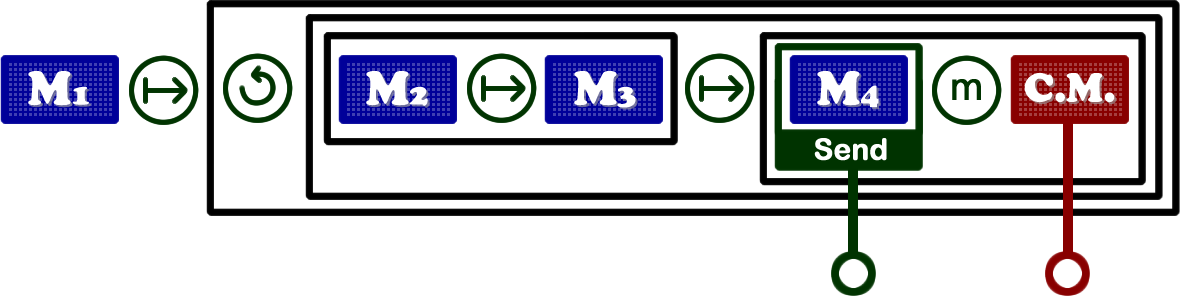
\includegraphics[width=0.6\linewidth]{example_1.png}
	}\\
	\subfloat[][Connecting \posl{} solvers to create \comstrs]{%
		\label{subfig:conn}
		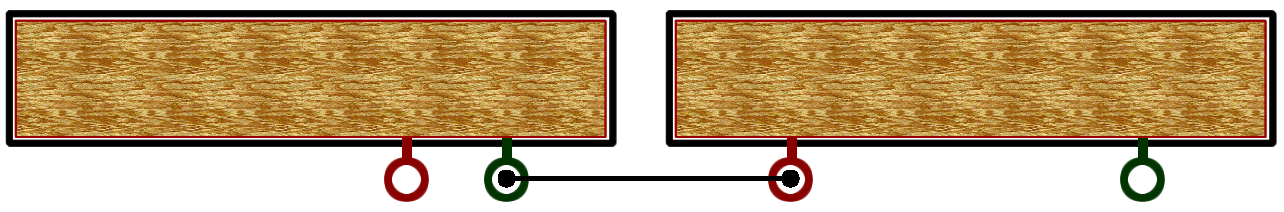
\includegraphics[width=0.6\linewidth]{conn.png}
	}
	\caption[]{Solver construction process using \posl}
	\label{fig:posl}
\end{figure}

%Once the solvers set is ready, the last step is to model the problem to solve. To do so, the user must follow the framework specification to implement the benchmark, respecting some requirements. The most important one is to implement a {\it cost function} computing the cost for a given configuration, i.e., an integer indicating how much the configuration violates the set of constraints. This integer equals zero if the configuration is a solution.

In the following sections all these steps are explained in details, but first, I explain how to model the target benchmark using \posl.

\section{Modeling the target benchmark}\label{sec:model}
%In this stage we explain formally our modeling process of a benchmark to be solved (or study) through \posl{}. We explain how to make use of the already existing models or to create new benchmarks using the basic layer of the framework in C++ making a proper usage of the object-oriented design.

\modified{Target problems are modelized in \posl{} using the C++ programing language, respecting some rules of the object-oriented design. First of all, the benchmark must inherit from the class \pclass{Benchmark} provided by \posl. This class does not have any method to override or implement, but it receives in its constructor three objects, instances from classes that the user must create, inheriting from \pclass{SolutionCostStrategy}, \pclass{RelativeCostStrategy} and \pclass{ShowStrategy} respectively. In these classes we write the most important functionalities of the benchmark model.}

\underline{\textbf{SolutionCostStrategy}}: \modified{In this class is implemented the strategy to compute the \textit{cost} of a configuration. \posl{} is based on improving step by step an initial configuration, tacking into account a \textit{cost function} provided by the user through the model (implementing the function \pmethod{solutionCost}{$dots$}). The kind of problems that \posl{} solves are the \CSPs{}, so this \textit{cost function} must be a function returning an integer taking into account the problem constraints. Given a configuration $s$, the \textit{cost function}, as a mandatory rule, must return 0 if and only if $s$ is a solution of the problem, i.e., $s$ aims all the problem constraints. An example of \textit{cost function} can be returning the number of violated constraints. However, the more \tet{expressive} is the function cost, the better the behavior of \posl{} is leading to the solution.}

The method to implement in this class is:

\begin{itemize}
\item \verb|int solutionCost(std::vector<int> & c)| $\rightarrow$ It computes the cost of a given configuration (\verb|c|).
\end{itemize}

\underline{\textbf{RelativeCostStrategy}}: \modified{In this classe the user implements the strategy to compute the \textit{cost} of a given configuration, with respect to another: the current one. If the user is able to compute the cost of a configuration, by knowing the performed changes with respect to the current configuration, the search process becomes more efficient, because this function is very often executed.}

The methods to implement in this class are:

\begin{itemize}
\item \verb|void initializeCostData(std::vector<int> & c)| $\rightarrow$ Initializes the information related to the cost (auxiliary data structures, the current configuration (\verb|c|), the current cost, etc.)
\item \verb|void updateConfiguration(std::vector<int> & c)| $\rightarrow$ Updates the information related to the cost.
\item \verb|int relativeSolutionCost(std::vector<int> & c)| $\rightarrow$ Returns the relative cost of the configuration \verb|c| with respect to the current configuration.
\item \verb|int currentCost()| $\rightarrow$ Property that returns the cost of the current configuration.
\item \verb|int costOnVariable(int variable_index)| $\rightarrow$ Returns a measure of how much some variable is contributing to the total cost of a configuration. % \tet{AMPLIAR}
\item \verb|int sickestVariable()| $\rightarrow$ Returns the variable contributing more to the cost.
\end{itemize}

\underline{\textbf{SolutionCostStrategy}}: \modified{This class represents the way a benchmark shows a configuration, in order to be clearer and to give more information about the structure. For example, a configuration of the instance 3--3--2 of the \sgp{} (see bellow for more details about this benchmark) can be written as follows:}

\begin{Verbatim}
[1, 2, 3, 4, 5, 6, 7, 8, 9, 3, 4, 5, 6, 7, 8, 9, 1, 2]
\end{Verbatim}

\modified{But this text is very difficult to read if the instance is bigger. For that reason, the user should implement this class in order to give more details and make easier the configuration read. For example, for the same instance of the problem, a solution is presented as follows:}

\begin{Verbatim}
Golfers: players-3, groups-3, weeks-2
6	8	7	
1	3	5	
4	9	2	
--
7	2	3	
4	8	1	
5	6	9	
--
\end{Verbatim}

The method to implement in this class is:

\begin{itemize}
\item \verb|std::string showSolution(std::shared_ptr<Solution> s)| $\rightarrow$ Returns a string to write in the standard output.
\end{itemize}

\modified{Once we have modelized the target benchmark, we can solve it through \posl{}. In the following sections we describe how to use this parallel-oriented language to solve \CSPs.}

\section{First stage: creating \posl's modules}\label{sec:1ststage}
There exist two types of basic modules in \posl: \INTROom{} and \INTROopch{}. A \om{} is basically a function and a \opch{} is also a function, but in contrast, it can receive information from two different sources: through input parameters or from outside, i.e., by communicating with a module from another solver.

\subsection{Computation module}

%In this sub-section we expose the definition and the characteristics and the details of the \om, and give some examples. We explain how to create new \oms{} using the basic layer of the framework.

A \om{} is the most basic and abstract way to define a piece of computation. It is a function which receives an instance of a \posl{} data type as input, then executes an internal algorithm, and returns an instance of a \posl{} data type as output. The input and output types will characterize the computation module signature. It can be dy\-na\-mi\-cally replaced by (or combined with) other computation modules, since they can be transmitted to other solvers working in parallel. They are joined through operators defined in Section~\ref{sec:2ndstage}.

\defname{Computation Module}{
A \om{} $Cm$ is a mapping defined by: 
\begin{equation}
\label{def:om}
Cm:I \rightarrow O
\end{equation}
}

where $I$ and $O$, for instance, can be independently a set of configurations, a set of sets of configurations, a set of values of some data type, etc.

Consider a local search meta-heuristic solver. One of its \oms{} can be the function returning the set of configurations composing the neighborhood of a given configuration:

\begin{equation*}
Cm_{neighborhood}:I_1\times I_2\times\dots\times I_n \rightarrow 2^{I_1\times I_2\times\dots\times I_n}
\end{equation*}

\noindent where $I_i$ represents the definition domains of each variable of the input confi\-gura\-tion.

Figure~\ref{fig:om} shows an example of \om: which receives a configuration $S$ and then computes the set $\mathcal{V}$ of its neighbor configurations $\left\{S^1, S^2, \dots, S^m\right\}$.

%\vspace{0.5cm}
\begin{figure}
	\centering	
	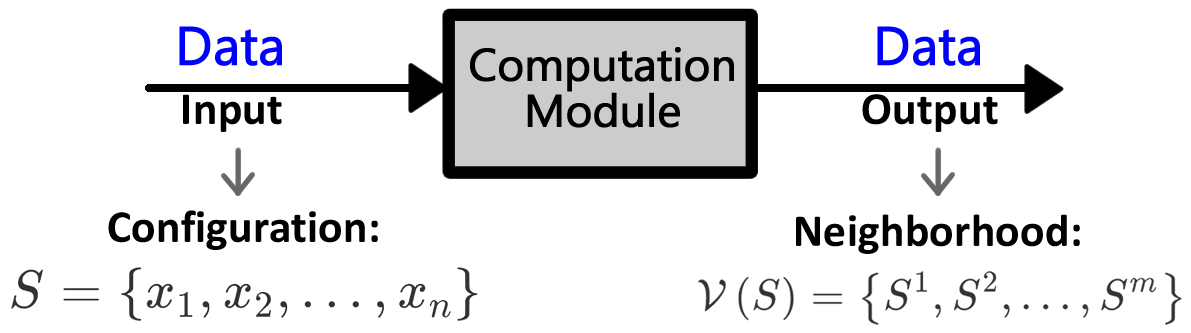
\includegraphics[width=0.7\linewidth]{OM.png}
	\caption{An example of a computation module computing a neighborhood}\label{fig:om}
\end{figure}

\subsubsection{Creating new \oms}
\label{subsubsec:creatingoms}

To create new \oms{} we use C++ programing language. \posl{} provides a hierarchy of data types to work with (see Appendix~\ref{app:diag}) and some abstract classes to inherit from, depending on the type of \om{} the user wants to create. These abstract classes represent {\it abstract} \oms{} and define a type of action to be executed. In the following we present the most important ones:

\begin{itemize}
\item \pclass{ACM\_FirstConfigurationGeneration} $\rightarrow$ Represents \oms{} returning a configuration, usually used for generating the starting configuration on local search meta-heuristics. The user must implement the method \pmethod{execute}{\pclass{ComputationData}} which returns a pointer to a \pclass{Solution}, that is, an object containing all the information concerning a partial solution (configuration, variable domains, etc.)
\item \pclass{ACM\_NeighborhoodFunction} $\rightarrow$ Represent \oms{} receiving a configuration as input and returning its neighborhood as output. The user must implement the method \pmethod{execute}{\pclass{Solution}} which returns a pointer to an object \pclass{Neighborhood}, containing a set of configurations which constitute the neighborhood of a given configuration, according to certain criteria. These configurations are efficiently stored in term of space.
\item \pclass{ACM\_SelectionFunction} $\rightarrow$ Represents \oms{} receiving a neighborhood as input and selecting a configuration from it as output. The user must implement the method \pmethod{execute}{\pclass{Neighborhood}} which returns a pointer to an object \pclass{DecisionPair}, containing two solutions: the current and the selected one.
\item \pclass{ACM\_DecisionFunction} $\rightarrow$ Represents \oms{} receiving a couple af configurations encapsulated into a \pclass{DecisionPair} object, and returning the configuration to be the current one for the next iteration. The user must implement the method \pmethod{execute}{\pclass{DecisionPair}} which returns a pointer to an object \pclass{Solution}.
\item \pclass{ACM\_ProcessingConfigurationFunction} $\rightarrow$ Represents \oms{} receiving a configuration and returning another configuration as result of some arrangement, like for example, a reset. The user must implement the method \pmethod{execute}{\pclass{Solution}} which returns a pointer to an object \pclass{Solution}.
\end{itemize}

\subsection{Communication modules}

%In this sub-section we expose the definition and the characteristics and the details of the \opch, and give some examples. We explain how to create new \opchs{} using the basic layer of the framework.

A \opch{} is the component managing the information reception in the communication between solvers (I talk about information transmission in Section~\ref{sec:2ndstage}). They can interact with \oms{} through operators (see Figure~\ref{fig:och}).

A \opch{} can receive two types of information from an external solver: data or \oms{}. It is important to notice that by sending/receiving \oms, I mean sending/receiving the required information to identify and being able to instantiate the \om. For instance, an integer identifier.

In order to distinguish from the two types of \opchs, I will call \INTROdopch{} the \opch{} responsible for the data reception (Figure~\ref{subfig:doch}), and \INTROoopch{} the one responsible for the reception and instantiation of \oms{} (Figure~\ref{subfig:ooch}).

\defname{Data Communication Module}{
A \emph{Data Communication Module} $Ch$ is a module that produces a mapping defined as follows: 
\begin{equation}
\label{def:dopench}
Ch:I\times \left\{D\cup \left\{NULL\right\}\right\} \rightarrow D \cup \left\{NULL\right\}
\end{equation}
No matter what the input $I$ is, it returns the information $D$ coming from an external solver.
}

\defname{Object Communication Module}{
	If we denote by $\mathbb{M}$ the space of all the \oms{} defined by Definition~\ref{def:om}, then an \emph{\oopch} $Ch$ is a module that produces and executes a \om{} coming from an external solver as follows:
	\begin{equation}
	\label{def:oopench}
	Ch:I\times\left\{\mathbb{M}\cup\left\{NULL\right\}\right\} \rightarrow O \cup \left\{NULL\right\}
	\end{equation}
It returns the output $O$ of the execution of the \om{} coming from an external solver, using $I$ as the input.
}%

\begin{figure}
	\centering
	\subfloat[][Data \opch]{
		\label{subfig:doch}
		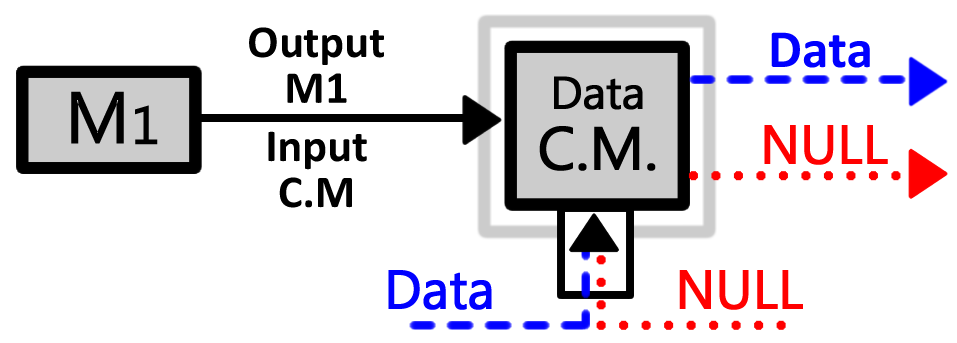
\includegraphics[width=0.4\linewidth]{D_OCh.png}
	}
	\hspace{0.05\textwidth}%
	\subfloat[][Object \opch]{%
		\label{subfig:ooch}
		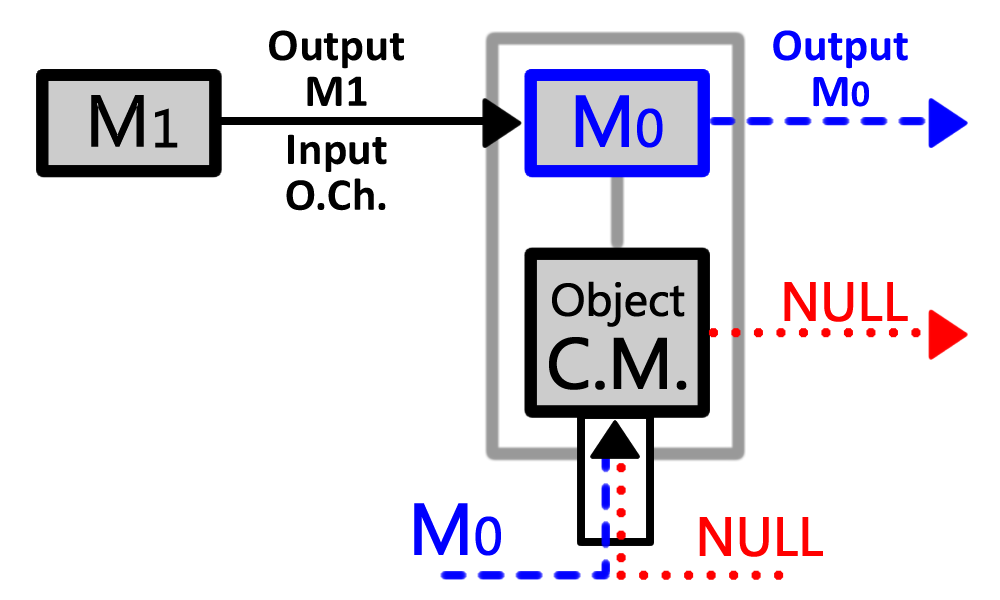
\includegraphics[width=0.4\linewidth]{O_OCh.png}
	}
	\caption[]{Communication module}
	\label{fig:och}
\end{figure}

Users can implement new computation and connection modules but \posl{} already contains many useful modules for solving a broad range of problems.

Due to the fact that \opchs{} receive information coming from outside without having control on them, it is necessary to define the {\it NULL} information, in order to denote the absence of information. If a Data Communication Module receives information, it is returned automatically. If a Object Communication Module receives a \om{}, it is instantiated and executed with the \opch's input and its result is returned. In both cases, if no available information exists (no communications performed), the \opch{} returns the {\it NULL} object.

\section{Second stage: assembling \posl's modules}\label{sec:2ndstage}
The modules mentioned above are grouped according to their signatures. An \textit{abstract module} is a module that represents all modules with the same signature. For example, the module showed in Figure~\ref{fig:om} is a \om{} based on an abstract module that receives a configuration and returns a neighborhood. %In that sense, an example of a concrete \om{} (or just \om{}) can be a function receiving a configuration, and returning a neighborhood constituted by $N$ configurations which only differ from the input configuration in one entry.

At this stage an \INTROas{} is coded using \posl{}. It takes abstract modules as {\it parameters} and combines them through operators. Through the \as, we can also decide which information to send to other solvers. % by using some operators to send the result of a computation module (see below). In the following we present a formal and more detailed specification of \posl{}'s operators. 

The \as{} is the solver's backbone. It joins the \oms{} and the \opchs{} coherently. It is independent from the \oms{} and \opchs{} used in the solver. It means that modules can be changed or modified during the execution, respecting the algorithm structure. Each time we combine some of them using \posl's operators, we are creating a \INTROcm. Here, we formally define the concept of \textit{module} and \INTROcm.

\begin{definition}
\label{def:module}
A {\bf module} is (Denoted by the letter $\mathcal{M}$):
\begin{enumerate}\renewcommand{\labelitemi}{\scriptsize$\blacksquare$}
\item a \om{}; or
\item a \opch{}; or
\item $\left[\text{OP } \mathcal{M}\right]$, which is the composition of a module $\mathcal{M}$ to be executed sequentially, returning an output depending on the nature of the unary operator \emph{OP}; or\label{subdef:seq_uni}
\item $\left[\mathcal{M}_1 \text{ OP } \mathcal{M}_2\right]$, which is the composition of two modules $\mathcal{M}_1$ and $\mathcal{M}_2$ to be executed sequentially, returning an output depending on the nature of the binary operator \emph{OP}; or\label{subdef:seq}
\item $\parallelexec{\mathcal{M}_1 \text{ OP } \mathcal{M}_2}$, which is the composition of two modules $\mathcal{M}_1$ and $\mathcal{M}_2$ to be executed, returning an output depending on the nature of the binary operator \emph{OP}. These two modules will be executed in parallel if and only if \emph{OP} supports parallelism, %(i.e. some modules will be executed sequentially although they were grouped this way); 
otherwise an exception is thrown.\label{subdef:par}
\end{enumerate}
$\mathbb{M}$ denotes the space of the modules, and we call \cms{} the composition of modules described in \ref{subdef:seq_uni}, \ref{subdef:seq} and/or \ref{subdef:par}.
\end{definition}

For a better understanding of Definition~\ref{def:module}, Figure~\ref{fig:cm} shows graphically  the structure of a \cm.

\begin{figure}[h]
	\centering
	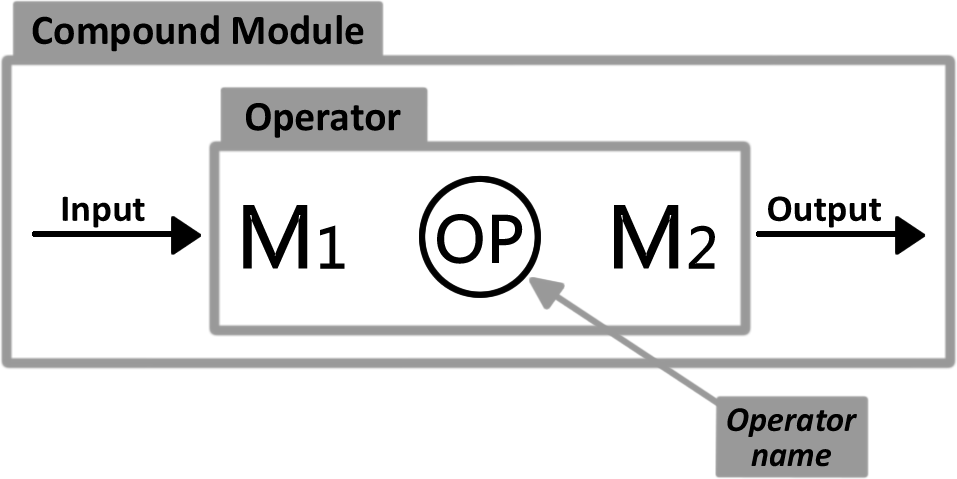
\includegraphics[width=0.5\linewidth]{cm.png}
	\caption[]{A \cm{} made of two modules $M_1$ and $M_2$}
	\label{fig:cm}
\end{figure}

As mentioned before, the \as{} is independent from the \oms{} and \opchs{} used in the solver. It means that one \as{} can be used to construct many different solvers, by implementing it with different modules. %(see below the related concept of \as{} instantiation). 
This is the reason why the \as{} is defined only using {abstract} modules. Formally, we define an \as{} as follows:

\defname{Abstract Solver}{
An \emph{Abstract Solver} $AS$ is a triple $\left(\mathbf{M},\mathcal{L}^m, \mathcal{L}^c\right)$, where: $\mathbf{M}$ is a \cm{} (also called \emph{root \cm{}}), $\mathcal{L}^m$ a list of abstract \oms{} appearing in $\mathcal{M}$, and $\mathcal{L}^c$ a list of \opchs{} appearing in $\mathcal{M}$.}

\Cms{}, and in particular the \textit{root} \cm{}, can be defined also as a context-free grammar as follows.

\begin{definition}\label{def:grammar} A {\bf \cm{}'s grammar} is the set $G_{POSL} = \left(\mathbf{V},\Sigma, \mathbf{S}, \mathbf{R}\right)$, where:
\begin{enumerate}\renewcommand{\labelitemi}{\scriptsize$\blacksquare$}
	\item $\mathbf{V} = \left\{CM, OP\right\}$ is the set of {\it variables},
	\item $\Sigma = \left\{\alpha, \beta, be, [, ], \lbk, \rbk_p, \lsendpar, \rsenddatapar, \rsendmodulepar, \circled{$\mapsto$},\circled{?},\cycop, \circled{$\rho$}, \circled{$\vee$}, \circled{$\wedge$}, \circled{M}, \circled{m}, \circled{$\shortdownarrow$}, \circled{$\cup$}, \circled{$\cap$}\right\}$ is the set of {\it terminals},
	\item $\mathbf{S} = \left\{CM\right\}$ is the set of {\it start variables},
	\item and $\mathbf{R} = $
		\begin{align*} 
		CM \produce & \alpha \OR \beta \OR \senddataop{CM} \OR \sendmoduleop{CM} \OR \left[OP\right] \OR \lbk OP\rbk_p\\
		OP \produce & CM \circled{$\mapsto$} CM \OR CM \circled{?} CM \OR CM \circled{$\rho$} CM \OR CM \circled{$\vee$} CM \OR CM \circled{$\wedge$} CM  \OR\\
		& CM \circled{M} CM \OR CM \circled{m} CM \OR CM \circled{$\shortdownarrow$} CM \OR CM \circled{$\cup$} CM \OR CM \circled{$\cap$} CM  \OR\\
		& \cycop \text{ be } CM%\left\{CM\right\}		
		\end{align*} is a set of {\it rules}
\end{enumerate} 
%For simplicity, we will use, from now on, the name of \emph{Module} to refer ether to an \module, to an \opch, or to a \cm.
\end{definition}

In the following, some of the concepts of Definition~\ref{def:grammar} are explained:
\begin{itemize}
	\item The variables $CM$ and $OP$ correspond to a \cm{} and an {\it operator}, respectively.
	\item The terminals $\alpha$ and $\beta$ represent a \om{} and a \opch{}, respectively.
	\item The terminal $be$ is a Boolean expression.
	\item The terminals $[\text{ } ], \parallelexec{\text{ }}$ are symbols for grouping and defining the way the involved \cms{} are executed. Depending on the nature of the operator, this can be either sequentially or in parallel:
	\begin{enumerate}\renewcommand{\labelitemi}{\scriptsize$\blacksquare$}
		\item $\left[\text{OP}\right]$: The involved operator will always executed sequentially.
		\item $\parallelexec{\text{OP}}$: The involved operator will be executed in parallel if and only if \emph{OP} supports parallelism. Otherwise, an exception is thrown.
	\end{enumerate}
	\item The terminals $\senddataop{.}, \sendmoduleop{.}$ are operators to send information to other solvers (explained bellow).
	\item All other terminals are \posl{} operators that are detailed later.
\end{itemize}

In the following we define \posl{} operators. For grouping modules, like in Definition~\ref{def:module}(\ref{subdef:seq}) and \ref{def:module}(\ref{subdef:par}), we will use $\left|OP\right|$ as a generic grouper. In order to help the reader to easily understand how to use operators, we use an example of a solver that we build step by step, while presenting the definitions.

%\begin{example}
%\mybox{Example}
\poslexample{
\posl{} creates solvers based on local search meta-heuristics algorithms. These algorithms have a common structure: \begin{inparaenum}[1.] \item They start by initializing some data structures (e.g., a \emph{tabu list} for \emph{Tabu Search}, a \emph{temperature} for \emph{Simulated Annealing}, etc.). \item An initial configuration $s$ is generated. \item A new configuration $s'$ is selected from the neighborhood $\mathcal{V}\left(s\right)$. \item If $s'$ is a solution for the problem $P$, then the process stops, and $s'$ is returned. Otherwise, the data structures are updated, and $s'$ is accepted or not for the next iteration, depending on a certain criterion. \end{inparaenum}
%An example of such data structure is the penalizing features of local optima in \emph{Guided Local Search} algorithm.

Abstract \oms{} composing local search meta--heuristics are:

\begin{list}{\boxed{Abstract\hspace{4pt}computation\hspace{4pt}module- \arabic{qcounter}~}}{\usecounter{qcounter}} \itemsep0em 
	\item $I$: Generating a configuration $s$
	\item $V$: Defining the neighborhood $\mathcal{V}\left(s\right)$
	\item $S$: Selecting $s' \in \mathcal{V}\left(s\right)$
	\item $A$: Evaluating an acceptance criterion for $s'$
\end{list}
} %\end{example}

The list of modules to be used in the examples have been presented. Now we present \posl{} operators.

\separation

\begin{definition}\label{op:seqexec}
$\circled{$\mapsto$}$ {\bf Sequential Execution Operator.} Let
\begin{enumerate}%\begin{inparaenum}[i)]
	\item $\mathcal{M}_1 : \mathcal{I}_1 \rightarrow \mathcal{O}_1$ and 
	\item $\mathcal{M}_2 : \mathcal{I}_2 \rightarrow \mathcal{O}_2$, 
\end{enumerate}%\end{inparaenum} 
be modules, where $\mathcal{O}_1 \subseteq \mathcal{O}_2$. Then the operation $\left|\mathcal{M}_1\circled{$\mapsto$} \mathcal{M}_2\right|$ defines the \cm{} $\mathcal{M}_{seq}$ as the result of executing $\mathcal{M}_1$ followed by executing $\mathcal{M}_2$:

\[
\mathcal{M}_{seq}:\mathcal{I}_1 \rightarrow \mathcal{O}_2
\]
\end{definition}

This is an example of an operator that does not support the execution of its involved \cms{} in parallel, because the input of the second \cm{} is the output of the first one.

\poslexample{
Coming back to the example, defined abstract \oms{} can be used to create a \cm{} that performs only one iteration of a local search, using the {\bf Sequential Execution} operator. We create a \cm{} to execute sequentially $I$ and $V$ (see Figure~\ref{subfig:ex_seq1}), then we create another \cm{} to execute sequentially the \cm{} already created and $S$ (see Figure~\ref{subfig:ex_seq2}), and finally this \cm{} and the \om{} $A$ are executed sequentially (see Figure~\ref{subfig:ex_seq3}). The \cm{} presented in Figure~\ref{subfig:ex_seq3} can be coded as follows:
$$\left[\left[\left[I\poslop{\mapsto}V\right]\poslop{\mapsto}S\right]\poslop{\mapsto}A\right]$$
In the figure, each rectangle is a \cm.
}

\begin{figure}[h]
	\centering
	\subfloat[][]{
		\label{subfig:ex_seq1}
		
\includegraphics[width=0.2\linewidth]{seq_1.png}
	}\hspace{0.05\linewidth}
	\subfloat[][]{%
		\label{subfig:ex_seq2}
		
\includegraphics[width=0.3\linewidth]{seq_2.png}
	}\\
	\subfloat[][]{%
		\label{subfig:ex_seq3}
		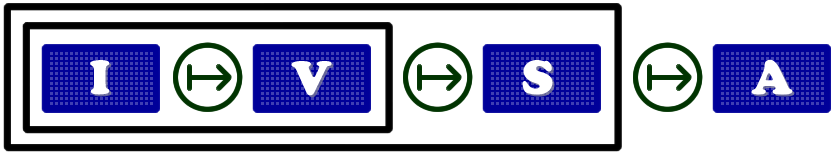
\includegraphics[width=0.4\linewidth]{seq_3.png}
	}
	\caption[]{Using {\bf sequential execution} operator}
	\label{fig:seq_example}
\end{figure}

\separation

The following operator is very useful to execute modules sequentially creating bifurcations, subject to some Boolean condition:

%---------------------------------------------------------
%-----   Conditional Execution Operator
%---------------------------------------------------------
\begin{definition}\label{op:conditional}
$\circled{?}$ {\bf Conditional Execution Operator} Let
\begin{enumerate}%\begin{inparaenum}[i)]
	\item $\mathcal{M}_1 : \mathcal{I} \rightarrow \mathcal{O}_1$ and  
	\item $\mathcal{M}_2 : \mathcal{I} \rightarrow \mathcal{O}_2$,
\end{enumerate}%\end{inparaenum} 
be modules. %, where $\mathcal{D}_1 = \mathcal{D}_2$. %and $\mathcal{I}_1 \subset \mathcal{I}_2$. 
Then the operation $\left|\mathcal{M}_1\circled{?}_{<cond>}\mathcal{M}_2\right|$ defines the \cm{} $\mathcal{M}_{cond}$ as result of the sequential execution of $\mathcal{M}_1$ if $<cond>$ is {\bf true} or $\mathcal{M}_2$, otherwise:

\[
\mathcal{M}_{cond}:\mathcal{I} \rightarrow \mathcal{O}_1 \cup \mathcal{O}_2 
\]
\end{definition}

\poslexample{
This operator can be used in the example if we want to execute two different {\it selection} \oms{} ($S_1$ and $S_2$) depending on certain criterion (see Figure~\ref{fig:cond_example}):
$$\left[\left[\left[I\poslop{\mapsto}V\right]\poslop{\mapsto}\left[S_1\poslop{?}S_2\right]\right]\poslop{\mapsto}A\right]$$
In examples we remove the clause $<cond>$ for simplification.
}

\begin{figure}[h]
	\centering	
	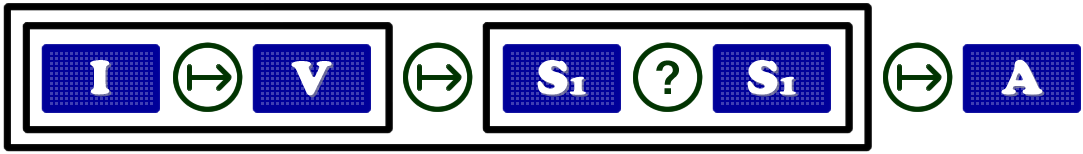
\includegraphics[width=0.5\linewidth]{cond.png}
	\caption{Using {\bf conditional execution} operator}\label{fig:cond_example}
\end{figure}

\separation

We can execute modules sequentially creating also cycles.

%---------------------------------------------------------
%-----   Cyclic Operator
%---------------------------------------------------------

\begin{definition}\label{op:cyclic}
$\cycop$ {\bf Cyclic Execution Operator} Let $\mathcal{M} : \mathcal{I} \rightarrow \mathcal{O}$ be a module, where $\mathcal{O} \subseteq \mathcal{I}$. Then, the operation $\left|\cycop_{<cond>}\mathcal{M}\right|$ defines the \cm{} $\mathcal{M}_{cyc}$ repeating sequentially the execution of $\mathcal{M}$ while $<cond>$ remains {\bf true}:

\[
\mathcal{M}_{cyc}:\mathcal{I} \rightarrow \mathcal{O} 
\]
\end{definition}

\poslexample{
Using this operator we can model a local search algorithm, by executing the {\it abstract} \om{} $I$ and then the other \oms{} ($V$, $S$ and $A$) cyclically, until finding a solution (\ie a configuration with cost equals to zero) (see Figure~\ref{fig:cyc_example}):
$$\left[I\poslop{\mapsto}\left[\cycop\left[\left[V\poslop{\mapsto}S\right]\poslop{\mapsto}A\right]\right]\right]$$
In the examples, we remove the clause $<cond>$ for simplification. 
}

\begin{figure}[h]
	\centering	
	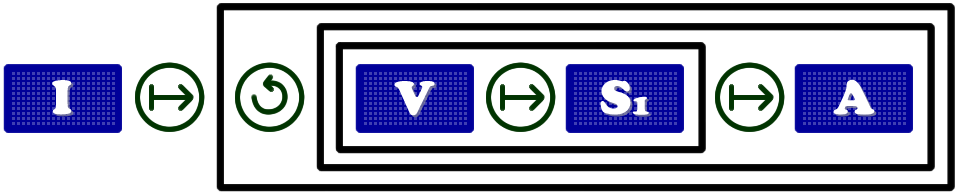
\includegraphics[width=0.5\linewidth]{cyc.png}
	\caption{Using {\bf cyclic execution} operator}\label{fig:cyc_example}
\end{figure}

\separation

%---------------------------------------------------------
%-----   Random Choice Operator
%---------------------------------------------------------
\begin{definition}\label{op:rho}
$\circled{$\rho$}$ {\bf Random Choice Operator} Let
\begin{enumerate}%\begin{inparaenum}[i)]
	\item $\mathcal{M}_1 : \mathcal{I} \rightarrow \mathcal{O}_1$ and  
	\item $\mathcal{M}_2 : \mathcal{I} \rightarrow \mathcal{O}_2$,
\end{enumerate}%\end{inparaenum} 
be modules. %, where $\mathcal{D}_1 = \mathcal{D}_2$, % and $\mathcal{I}_1 \subset \mathcal{I}_2$, 
and a real value $\rho \in (0,1)$. Then the operation $\left|M_1\circled{$\rho$}\mathcal{M}_2\right|$ defines the \cm{} $\mathcal{M}_{rho}$ executing $\mathcal{M}_1$ with probability $\rho$, or executing $\mathcal{M}_2$ with probability $(1-\rho)$:

\[
\mathcal{M}_{rho}:\mathcal{I} \rightarrow \mathcal{O}_1 \cup \mathcal{O}_2 
\]
\end{definition}

\poslexample{
In the example we can create a \cm{} to execute two {\it abstract} \oms{} $A_1$ and $A_2$ following certain probability $\rho$ using the {\bf random choice} operator as follows (see Figure~\ref{fig:rho_example}):
$$\left[I\poslop{\mapsto}\left[\cycop\left[\left[V\poslop{\mapsto}S\right]\poslop{\mapsto}\left[A_1\poslop{\rho}A_2\right]\right]\right]\right]$$
}

\begin{figure}[h]
	\centering	
	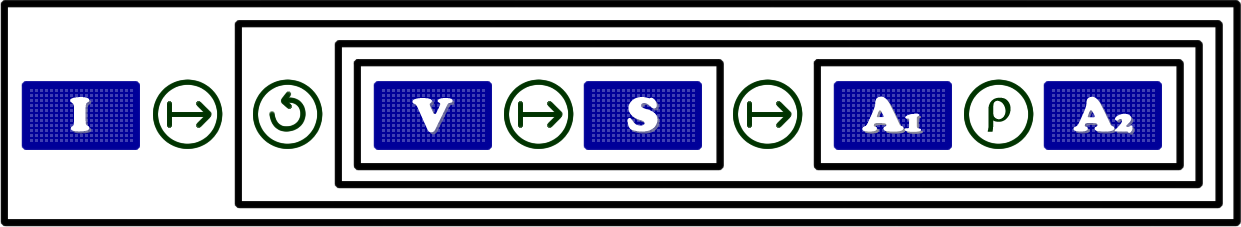
\includegraphics[width=0.6\linewidth]{rho.png}
	\caption{Using {\bf random choice} operator}\label{fig:rho_example}
\end{figure}

\separation

The following operator is very useful if the user needs to use a \opch{} inside an \as{}. As explained before, if a \opch{} does not receive any information from another solver, it returns {\it NULL}. This may cause the undesired termination of the solver if this case is not correctly handled. Next, we introduce the \textbf{Not {\it NULL} Execution Operator} and illustrate how to use it in practice with an example.

%---------------------------------------------------------
%-----   Not Null Operator
%---------------------------------------------------------
\begin{definition}\label{op:or}
$\circled{$\vee$}$ {\bf Not {\it NULL} Execution Operator} Let
\begin{enumerate}%\begin{inparaenum}[i)]
	\item $\mathcal{M}_1 : \mathcal{I} \rightarrow \mathcal{O}_1$ and  
	\item $\mathcal{M}_2 : \mathcal{I} \rightarrow \mathcal{O}_2$,
\end{enumerate}%\end{inparaenum} 
be modules. %, where $\mathcal{D}_1 = \mathcal{D}_2$. % and $\mathcal{I}_1 \subset \mathcal{I}_2$. 
Then, the operation $\left|\mathcal{M}_1\circled{$\vee$}\mathcal{M}_2\right|$ defines the \cm{} $\mathcal{M}_{non}$ that executes $\mathcal{M}_1$ and returns its output if it is not {\it NULL}, or executes $\mathcal{M}_2$ and returns its output otherwise:

\[
\mathcal{M}_{non}:\mathcal{I} \rightarrow \mathcal{O}_1 \cup \mathcal{O}_2 
\]
\end{definition}

\poslexample{Let us consider a slightly more complex example: when applying the acceptance criterion, suppose that we want to receive a configuration from other solver to combine the \om{} $A$ with a \opch:

\begin{list}{\boxed{Communication\hspace{4pt}module- \arabic{qcounter}:~}}{\usecounter{qcounter}} \itemsep0em
	\item $C.M.$: Receiving a configuration.\label{struct:opch}
\end{list}

Figure~\ref{fig:2difBeh} shows how to combine a \opch{} with the \om{} $A$ through the operator $\circled{$\vee$}$. Here, the \om{} $A$ will be executed as long as the \opch{} remains \textit{NULL}, i.e., there is no information coming from outside. This behavior is represented in Figure~\ref{subfig:beh1} by the blue lines. If some data has been received through the \opch, the later is executed instead of the module $A$, represented in Figure~\ref{subfig:beh2} by orange lines. 
The code can be written as follows:
$$\left[I\poslop{\mapsto}\left[\cycop\left[\left[V\poslop{\mapsto}S\right]\poslop{\mapsto}\left[C.M.\poslop{\vee}A\right]\right]\right]\right]$$
}

\begin{figure}[h]
\centering
\subfloat[][The solver executes the computation module {\bf A} if no information is received through the connection module]{
	\label{subfig:beh1}
	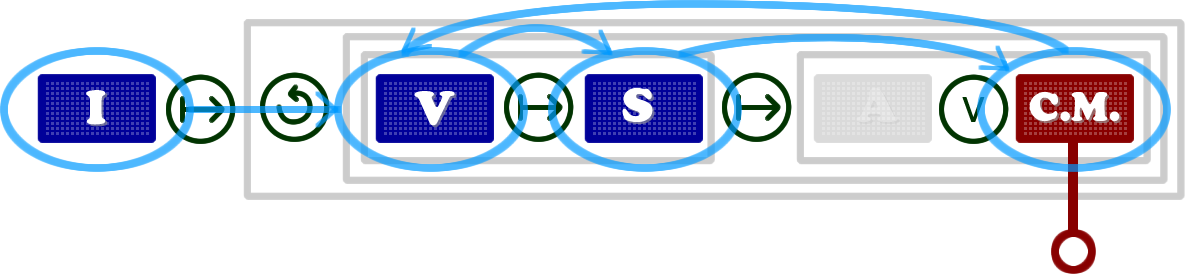
\includegraphics[width=0.6\linewidth]{muta2_v4.png}
}\\
%\hspace{0.05\textwidth}%
\subfloat[][The solver uses the information coming from an external solver]{%
	\label{subfig:beh2}
	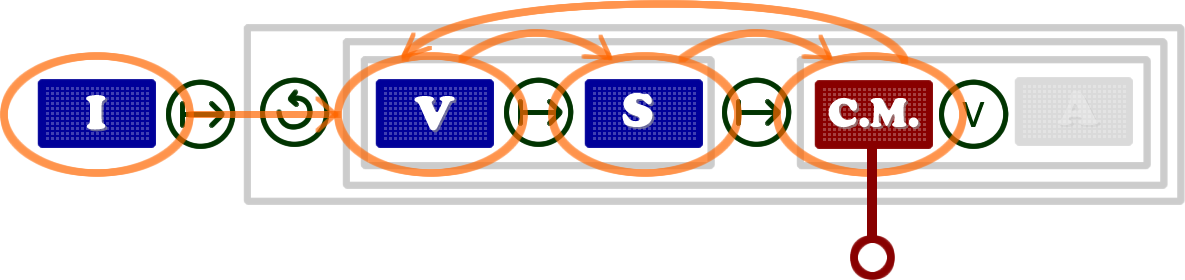
\includegraphics[width=0.6\linewidth]{muta1_v4.png}
}
\caption[]{Two different behaviors within the same solver}
\label{fig:2difBeh}
\end{figure}

\separation

The operator that we have just defined is a {\it short-circuit} operator. It means that if the first argument (module) does not return {\it NULL}, the second will not be executed. \posl{} provides another operator with the same functionality but not {\it short-circuit}. This operator is necessary if the user wants a side effect by always executing the second module also.

%---------------------------------------------------------
%-----   BOTH Operator
%---------------------------------------------------------

\begin{definition}\label{op:and}
$\circled{$\wedge$}$ {\bf {\it BOTH} Execution Operator} Let 
\begin{enumerate}%\begin{inparaenum}[i)]
	\item $\mathcal{M}_1 : \mathcal{I} \rightarrow \mathcal{O}_1$ and  
	\item $\mathcal{M}_2 : \mathcal{I} \rightarrow \mathcal{O}_2$,
\end{enumerate}%\end{inparaenum} 
be modules. %, where $\mathcal{D}_1 \subseteq \mathcal{D}_2$. % and $\mathcal{I}_1 \subset \mathcal{I}_2$. 
Then the operation $\left|\mathcal{M}_1\circled{$\wedge$}\mathcal{M}_2\right|$ defines the \cm{} $\mathcal{M}_{both}$ that executes both $\mathcal{M}_1$ and $\mathcal{M}_2$, then returns the output of $\mathcal{M}_1$ if it is not {\it NULL}, or the output of $\mathcal{M}_2$ otherwise:

\[
\mathcal{M}_{both}:\mathcal{I} \rightarrow \mathcal{O}_1 \cup \mathcal{O}_2 
\]
\end{definition}

\separation

In the following we introduce the concepts of {\it cooperative parallelism} and {\it competitive parallelism}. We say that cooperative parallelism exists when two or more processes are running separately, and the general result will be some combination of the results of at least some involved processes (e.g. Definitions~\ref{op:min} and~\ref{op:max}). On the other hand, competitive parallelism arise when the general result comes from an unique process, usialy the one finishing first (e.g. Definition~\ref{op:race}).

%---------------------------------------------------------
%-----   MIN Operator
%---------------------------------------------------------

\begin{definition}\label{op:min}
$\circled{m}$ {\bf Minimum Operator } Let
\begin{enumerate}%\begin{inparaenum}[i)]
	\item $\mathcal{M}_1 : \mathcal{I} \rightarrow \mathcal{O}_1$ and  
	\item $\mathcal{M}_2 : \mathcal{I} \rightarrow \mathcal{O}_2$,
\end{enumerate}%\end{inparaenum} 
be modules. %, where $\mathcal{D}_1 \subseteq \mathcal{D}_2$. %and $\mathcal{I}_1 \subset \mathcal{I}_2$. 
Let also $o_1$ and $o_2$ be the outputs of $\mathcal{M}_1$ and $\mathcal{M}_2$, respectively. Assume that there exists a total order in $O_1 \cup O_2$ where the object \emph{NULL} is the greatest value. Then the operation $\left|\mathcal{M}_1\circled{m}\mathcal{M}_2\right|$ defines the \cm{} $\mathcal{M}_{min}$ that executes $\mathcal{M}_1$ and $\mathcal{M}_2$, and returns $\min\left\{o_1,o_2\right\}$:

\[
\mathcal{M}_{min}:\mathcal{I} \rightarrow \mathcal{O}_1 \cup \mathcal{O}_2 
\]
\end{definition}

\separation

Similarly we define the \textbf{Maximum} operator:

%---------------------------------------------------------
%-----   MAX Operator
%---------------------------------------------------------

\begin{definition}\label{op:max}
$\circled{M}$ {\bf Maximum Operator} Let
\begin{enumerate}%\begin{inparaenum}[i)]
	\item $\mathcal{M}_1 : \mathcal{I} \rightarrow \mathcal{O}_1$ and  
	\item $\mathcal{M}_2 : \mathcal{I} \rightarrow \mathcal{O}_2$,
\end{enumerate}%\end{inparaenum} 
be modules. %, where $\mathcal{D}_1 \subseteq \mathcal{D}_2$. %and $\mathcal{I}_1 \subset \mathcal{I}_2$. 
Let also $o_1$ and $o_2$ be the outputs of $\mathcal{M}_1$ and $\mathcal{M}_2$, respectively. Assume that there exists a total order in $O_1 \cup O_2$ where the object \emph{NULL} is the smallest value. Then the operation $\left|\mathcal{M}_1\circled{M}\mathcal{M}_2\right|$ defines the \cm{} $\mathcal{M}_{max}$ that executes $\mathcal{M}_1$ and $\mathcal{M}_2$, and returns $\max\left\{o_1,o_2\right\}$:

\[
\mathcal{M}_{max}:\mathcal{I} \rightarrow \mathcal{O}_1 \cup \mathcal{O}_2 
\]
\end{definition}

\poslexample{The {\bf minimum operator} can be applied in the previews example to obtain an interesting behavior: When applying the acceptance criteria, suppose that we want to receive a configuration from another solver, to compare it with ours and select the one with the lowest cost. We can do that by applying the $\circled{m}$ operator to combine the \om{} $A$ with a \opch{} $C.M.$ (see Figure\ref{fig:min_example}):
$$\left[I\poslop{\mapsto}\left[\cycop\left[\left[V\poslop{\mapsto}S\right]\poslop{\mapsto}\lbk A\poslop{m}C.M.\rbk_p\right]\right]\right]$$
Notice that in this example, we can use the grouper $\lbk .\rbk_p$ since the {\bf minimum operator} supports parallelism.}

\begin{figure}[h]
	\centering	
	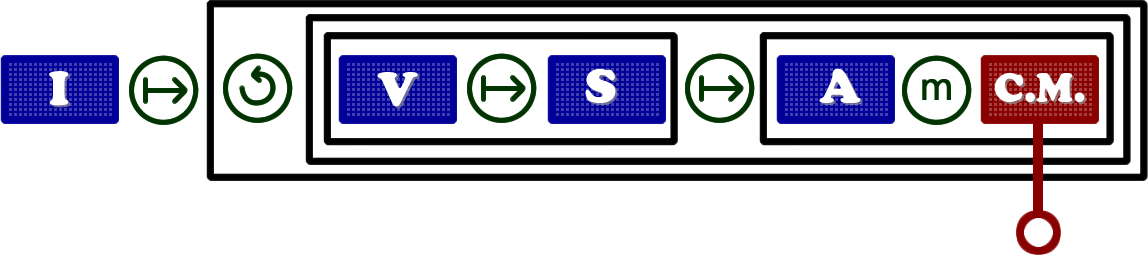
\includegraphics[width=0.6\linewidth]{min.png}
	\caption{Using {\bf minimum} operator}\label{fig:min_example}
\end{figure}

\separation

%---------------------------------------------------------
%-----   Race Operator
%---------------------------------------------------------

\begin{definition}\label{op:race}
$\circled{$\shortdownarrow$}$ {\bf Race Operator} Let 
\begin{enumerate}%\begin{inparaenum}[i)]
	\item $\mathcal{M}_1 : \mathcal{I} \rightarrow \mathcal{O}_1$ and  
	\item $\mathcal{M}_2 : \mathcal{I} \rightarrow \mathcal{O}_2$,
\end{enumerate}%\end{inparaenum} 
be modules. %, where $\mathcal{I}_1 \subseteq \mathcal{I}_2$ and $\mathcal{O}_1 \subset \mathcal{O}_2$. 
Then the operation $\left|\mathcal{M}_1\circled{$\shortdownarrow$}\mathcal{M}_2\right|$ defines the \cm{} $\mathcal{M}_{race}$ that executes both modules $\mathcal{M}_1$ and $\mathcal{M}_2$, and returns the output of the module ending first:

\[
\mathcal{M}_{race}:\mathcal{I} \rightarrow \mathcal{O}_1 \cup \mathcal{O}_2 
\]
\end{definition}

\poslexample{Sometimes nighborhood functions are slow depending on the configuration. In that case two neighborhood \oms{} can be executed and we take into account the output of the module ending first (see Figure\ref{fig:race_example}):
$$\left[I\poslop{\mapsto}\left[\cycop\left[\left[\lbk V_1\poslop{\shortdownarrow}V_2\rbk_p\poslop{\mapsto}S\right]\poslop{\mapsto}\lbk A\poslop{m}C.M.\rbk_p\right]\right]\right]$$}

\begin{figure}[h]
	\centering	
	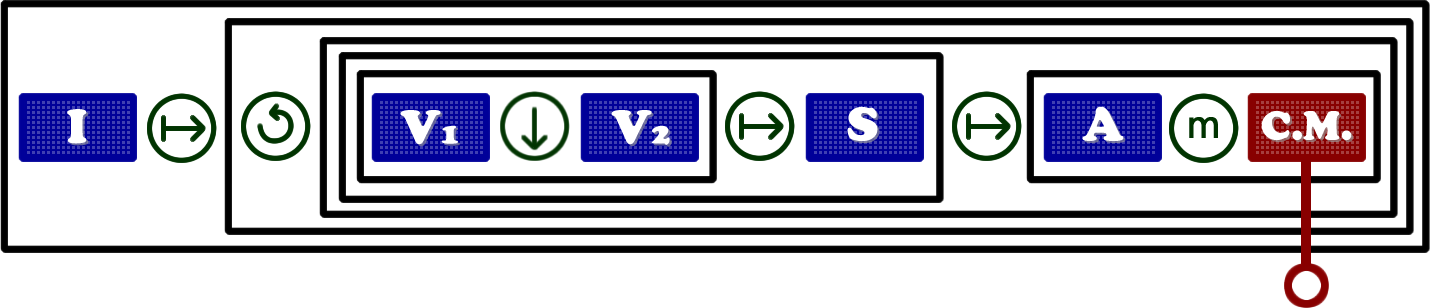
\includegraphics[width=0.7\linewidth]{race.png}
	\caption{Using {\bf race} operator}\label{fig:race_example}
\end{figure}

\separation

Some \posl's data types are related to sets, like neighborhoods. For that reason, it is useful to define operators to handle that kind of data. Although at this moment \posl{} is designed only to create solvers based on local-search meta-heuristic, is was conceived to be able to create population-based solvers as a future direction. In that sens, these operators are also useful.

\begin{definition}\label{op:union}
$\circled{$\cup$}$ {\bf Union Operator} Let 
\begin{enumerate}%\begin{inparaenum}[i)]
	\item $\mathcal{M}_1 : \mathcal{I} \rightarrow \mathcal{O}_1$ and  
	\item $\mathcal{M}_2 : \mathcal{I} \rightarrow \mathcal{O}_2$,
\end{enumerate}%\end{inparaenum} 
be modules. %, where $\mathcal{D}_1 \subseteq \mathcal{D}_2$. %and $\mathcal{I}_1 \subset \mathcal{I}_2$. 
Let also the sets $V_1$ and $V_2$ be the outputs of $\mathcal{M}_1$ and $\mathcal{M}_2$, respectively. Then the operation $\left|\mathcal{M}_1\circled{$\cup$}\mathcal{M}_2\right|$ defines the \cm{} $\mathcal{M}_{\cup}$ that executes both modules $\mathcal{M}_1$ and $\mathcal{M}_2$, and returns $V_1\cup V_2$:

\[
\mathcal{M}_{\cup}:\mathcal{I} \rightarrow \mathcal{O}_1 \cup \mathcal{O}_2
\]
\end{definition}

\separation

Similarly we define the operators \textbf{Intersection} and \textbf{Subtraction}:

\begin{definition}\label{op:intersec}
$\circled{$\cap$}$ {\bf Intersection Operator} Let 
\begin{enumerate}%\begin{inparaenum}[i)]
	\item $\mathcal{M}_1 : \mathcal{I} \rightarrow \mathcal{O}_1$ and  
	\item $\mathcal{M}_2 : \mathcal{I} \rightarrow \mathcal{O}_2$,
\end{enumerate}%\end{inparaenum} 
be modules. %, where $\mathcal{D}_1 \subseteq \mathcal{D}_2$. % and $\mathcal{I}_1 \subset \mathcal{I}_2$. 
Let also the sets $V_1$ and $V_2$ be the outputs of $\mathcal{M}_1$ and $\mathcal{M}_2$, respectively. Then the operation $\left|\mathcal{M}_1\circled{$\cap$}\mathcal{M}_2\right|$ defines the \cm{} $\mathcal{M}_{\cap}$ that executes both modules $\mathcal{M}_1$ and $\mathcal{M}_2$, and returns $V_1\cap V_2$:

\[
\mathcal{M}_{\cap}:\mathcal{I} \rightarrow \mathcal{O}_1 \cup \mathcal{O}_2
\]
\end{definition}

\separation

\begin{definition}\label{op:subst}
$\circled{$\setminus$}$ {\bf Subtraction Operator} Let 
\begin{enumerate}%\begin{inparaenum}[i)]
	\item $\mathcal{M}_1 : \mathcal{I} \rightarrow \mathcal{O}_1$ and  
	\item $\mathcal{M}_2 : \mathcal{I} \rightarrow \mathcal{O}_2$,
\end{enumerate}%\end{inparaenum} 
be modules. %, where $\mathcal{D}_1 \subseteq \mathcal{D}_2$. % and $\mathcal{I}_1 \subset \mathcal{I}_2$. 
Let also $V_1$ and $V_2$ be the outputs of $\mathcal{M}_1$ and $\mathcal{M}_2$, respectively. Then the operation $\left|\mathcal{M}_1\circled{$\setminus$}\mathcal{M}_2\right|$ defines the \cm{} $\mathcal{M}_{\setminus}$ that executes both modules $\mathcal{M}_1$ and $\mathcal{M}_2$, and returns $V_1 \setminus V_2$:

\[
\mathcal{M}_{\setminus}:\mathcal{I} \rightarrow \mathcal{O}_1
\]
\end{definition}

\separation

Now, we define the operators which allow to send information to other solvers. Two types of information can be sent: 
\begin{inparaenum}[i)]
	\item the output of the \om{} as result of its execution, or 
	\item the \om{} itself.
\end{inparaenum} This feature is very useful in terms of sharing behaviors between solvers.

\begin{definition}\label{op:osend}
$\senddataop{.}$ {\bf Sending Data Operator} Let $\mathcal{M} : \mathcal{I} \rightarrow \mathcal{O}$ be a module. Then the operation $\left|\senddataop{\mathcal{M}}\right|$ defines the \cm{} $\mathcal{M}_{sendD}$ that executes the module $\mathcal{M}$ and sends its output to a \opch:

\[
\mathcal{M}_{sendD}:\mathcal{I} \rightarrow \mathcal{O}
\]
\end{definition}

\separation

Similarly we define the \textbf{Send Module} operator:

\begin{definition}\label{op:msend}
$\sendmoduleop{.}$ {\bf Sending Module Operator} Let $\mathcal{M} : \mathcal{I} \rightarrow \mathcal{O}$ be a module. Then the operation $\left|\sendmoduleop{\mathcal{M}}\right|$ defines the \cm{} $\mathcal{M}_{sendM}$ that executes the module $\mathcal{M}$, then returns its output and sends the module itself to a \opch:

\[
\mathcal{M}_{sendM}:\mathcal{I} \rightarrow \mathcal{O}
\]
\end{definition}

\poslexample{In the following example, we use one of the \cms{} already presented in the previews examples, using a \opch{} to receive a configuration (see Figure~\ref{subfig:receiver_example}):  
$$\left[I\poslop{\mapsto}\left[\cycop\left[\left[V\poslop{\mapsto}S\right]\poslop{\mapsto}\lbk A\poslop{m}C.M.\rbk_p\right]\right]\right]$$

We also build another, as its complement: sending the accepted configuration to outside, using the {\bf sending data operator} (see Figure\ref{subfig:sender_example}):
$$\left[I\poslop{\mapsto}\left[\cycop\left[\left[V\poslop{\mapsto}S\right]\poslop{\mapsto}\senddataop{A}\right]\right]\right]$$

In the Section~\ref{sec:4thstage} we explain how to connect solvers to each other.
}

\begin{figure}[h]
\centering
\subfloat[][]{
	\label{subfig:receiver_example}
	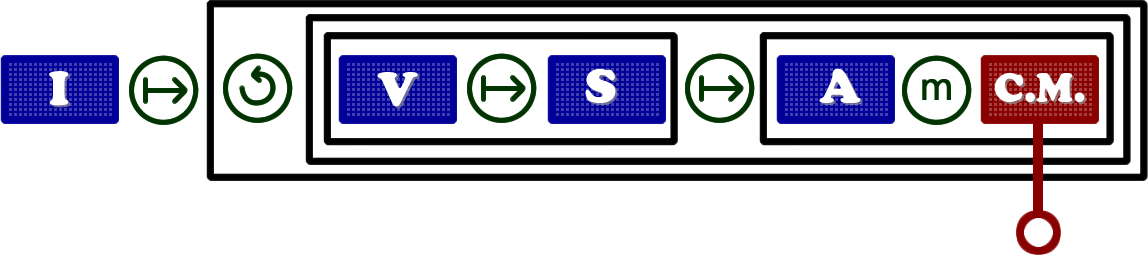
\includegraphics[width=0.6\linewidth]{min.png}
}\\
\subfloat[][]{%
	\label{subfig:sender_example}
	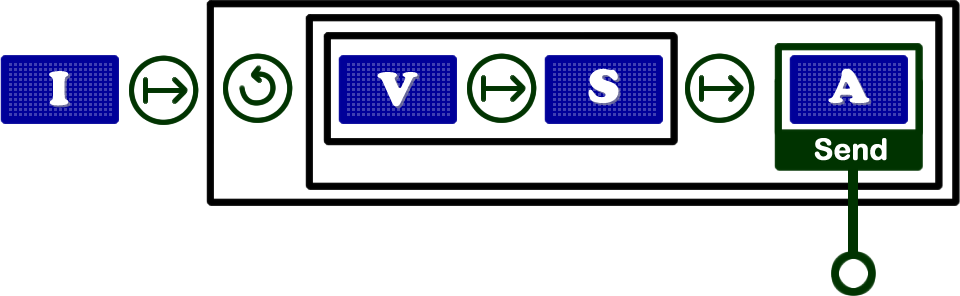
\includegraphics[width=0.6\linewidth]{send.png}
}
\caption[]{Sender and receiver behaviors}
\label{fig:send_recv}
\end{figure}

Sending \ms{} through this operator is performed by sending an identifier, in the case of \oms, or the corresponding \posl{} code in the case of \cms. The receptor \dopch{} creates the \m, executes it and returns its output. There exists other ways to do this task more efficiently, for example, compiling modules in a pre--processing stage and store them in memory, to be executed afterwards by sending only the reference. However, \posl{} does it this way, because it was thought to be able to apply learning techniques to the received modules in the future, and to adapt them to the experience of the solver during the search.

\separation

Once all desired abstract modules are linked together with operators, we obtain the root \cm{}, i.e., the algorithmic part of an \as. To implement a concrete solver from an \as, one must instantiate each abstract module with a concrete one respecting the required signature. From the same \as, one can implement many different concrete solvers simply by instantiating abstract modules with different concrete modules.

An \as{} is declared as follows: after declaring the \mbox{\tet{\bf \as}}'s name, the first line defines the list of abstract \oms, the second one the list of abstract \opchs, then the algorithm of the solver is defined as the solver's body (the root \cm{} $\mathbf{M}$), between \mbox{\tet{\bf begin}} and \mbox{\tet{\bf end}}.

An \as{} can be declared through the  simple regular expression:

\begin{center}
\tet{\bf abstract solver} {\it name} \tet{\bf computation}: $\mathcal{L}^m$ (\tet{\bf communication}: $\mathcal{L}^c$)? \tet{\bf begin} $\mathbf{M}$ \tet{\bf end}
\end{center}

where:
\begin{itemize}
\item {\it name} is the identifier of the \as{}, 
\item $\mathcal{L}^m$ is the list of abstract \oms{},
\item $\mathcal{L}^c$ is the list of abstract \opchs{}, and
\item $\mathbf{M}$ is the root \cm.
\end{itemize}

For instance, Algorithm~\ref{algo:as_example} illustrates the abstract solver corresponding to Figure~\ref{subfig:sender_example}.% Figure~\ref{subfig:as}.

\begin{algorithm}[H]
\dontprintsemicolon
\SetNoline
\SetKwProg{myproc}{}{}{}
\myproc{\tet{\bf abstract solver} as\_01\;
\tet{\bf computation} : $I, V, S, A$ \; 
\tet{\bf connection}: $C.M.$}{
	\Begin{
		$I\poslop{\mapsto}$
		\whileinline{$\left(\textbf{\Iter < } K_1\right)$}{
			$\left[V\poslop{\mapsto}S\poslop{\mapsto}\senddataop{A}\right]$ %\left[C.M.\poslop{m} \senddataop{A}\right]\right]$
		}
	}
}
\caption{\posl{} pseudo-code for the \as{} presented in Figure~\ref{subfig:sender_example}}\label{algo:as_example}
%\caption{\posl{} pseudo-code for the \as{} presented in Figure~\ref{subfig:as}}\label{algo:as_example}
\end{algorithm}	

\section{Third stage: creating \posl{} solvers}\label{sec:3rdstage}
%With operation modules and open channels already assembled through the \as, we can create solvers by instantiating modules. \posl{} provides an environment to this end and we present the procedure to use it.

%With \module s, \opch s and \cstr{} defined, we can create solvers by instantiating the declared components. \af{} provides an environment to this end, presented in Algorithm~\ref{algo:solver_def}, where $m_i$ and $ch_i$ represent the instances of the \module s and the instances of the \opch s to be passed by parameters to the \cstr{} $St$.

With \bothmodules{} composing an \as, one can create solvers by instantiating \ms. This is simply done by specifying that a given \mbox{\tet{\bf solver}} must \mbox{\tet{\bf implements}} a given \as, followed by the list of \omprefix{} then \opchs{}. These modules must match signatures required by the \as. Algorithm~\ref{algo:solver_def} implements Algorithm~\ref{algo:as_example} by instantiating modules shown in Figure~\ref{fig:2difBeh}.

\begin{algorithm}[H]
\dontprintsemicolon
\SetNoline
\SetKwProg{myproc}{}{}{}
%\myproc{
\tet{\bf solver} solver\_01 \tet{\bf implements} as\_01\;
\tet{\bf computation} : $I_{rand}, V_{std}, S_{best}, A_{alw}$ \; 
\tet{\bf connection}: $CM_{last}$\; %}{
%	\Begin{
%	}
%}
\caption{An instantiation of the \as{} presented in Algorithm~\ref{algo:as_example}}\label{algo:solver_def}
\end{algorithm}

Algorithm~\ref{algo:solver_def} is just an example of a solver instantiation, using some \oms{} provided by \posl{}, that are used and explained in details in the Chapter~\ref{chap:expe} of this document:
\begin{itemize}
\item $I_{rand}$ creates a random configuration.
\item $V_{std}$ creates a neighborhood of a given configuration, changing one element at a time.
\item $S_{best}$ selects the configuration of a neighborhood with the lowest cost.
\item $A_{alw}$ always accepts the incoming configuration.
\item $CM_{last}$ returns the last configuration arrived, if at the time of its execution, there is more than one configuration waiting to be received. 
\end{itemize}

\section{Forth stage: connecting solvers}\label{sec:4thstage}
Once a set of solvers is created, the last stage is to connect them to each other. Up to this point, solvers are disconnected, but they are ready to establish the communication. \posl{} provides tools  to the user to easily define cooperative strategies based on communication jacks and outlets. The pool of (concrete) connected solvers to be executed in parallel to solve a problem is called a \INTROsoset{}. 

%In the following we present two important concepts necessary to formalize \INTROcommoper.

\begin{definition}\label{def:comm_jack}
{\bf Communication Jack} Let $\mathcal{S}$ be a solver and a module $\mathcal{M}$. Then the operation $\mathcal{S}\cdot\mathcal{M}$ opens an outgoing connection from the solver $\mathcal{S}$, sending either 
\begin{inparaenum}[a)]
	\item the output of $\mathcal{M}$, if a sending data operator is applied to $\mathcal{M}$, as presented in Definition~\ref{op:osend}, or
	\item $\mathcal{M}$ itself, if a sending module operator is applied to $\mathcal{M}$, as presented in Definition~\ref{op:msend}.
\end{inparaenum}
\end{definition} 

\begin{definition}\label{def:comm_outlet}
{\bf Communication Outlet} Let $\mathcal{S}$ be a solver and a \opch{} $\mathcal{CM}$. Then, the operation $\mathcal{S}\cdot\mathcal{CM}$ opens an ingoing connection to the solver $\mathcal{S}$, receiving either 
\begin{inparaenum}[a)]
	\item the output of some \om{}, if $\mathcal{CM}$ is a \dopch{}, or
	\item a \om{}, if $\mathcal{CM}$ is an \oopch.
\end{inparaenum}
\end{definition} 

\separation

The communication is established by following the following rules guideline:
\begin{enumerate}%\begin{inparaenum}
	\item Each time a solver sends any kind of information by using a {\it sending} operator, it creates a \INTROjack.
	\item Each time a solver defines a \opch, it creates a \INTROoutlet. 
	\item Solvers can be connected to each other by linking \jacks{} to \outlets.
\end{enumerate} %\end{inparaenum}

%With the operator $(\cdot)$ we can have access to \oms{} sending information and to the \opch's names in a solver. 
%For example: $Solver_0\cdot \mathcal{M}$ provides access to the \om{} $\mathcal{M}$ in $Solver_0$ if and only if it is affected by a {\it sending} operator, and $Solver_1\cdot CM$ provides access to the \opch{} $CM$ in $Solver_1$.

Following, we define \textit{connection operators} that \posl{} provides.

\begin{definition}\label{op_conn:1to1}
\onetoone {\bf Connection One-to-One Operator} Let 
\begin{enumerate}
\item $\mathcal{J} = \left[\mathcal{S}_0\cdot \mathcal{M}_0, \mathcal{S}_1\cdot \mathcal{M}_1,\dots, \mathcal{S}_{N-1}\cdot \mathcal{M}_{N-1}\right]$ be the list of \jacks, and
\item $\mathcal{O} = \left[\mathcal{Z}_0\cdot \mathcal{CM}_0, \mathcal{Z}_1\cdot \mathcal{CM}_1,\dots, \mathcal{Z}_{N-1}\cdot \mathcal{CM}_{N-1}\right]$ be the list of \outlets{}
\end{enumerate} Then the operation 
\[
\mathcal{J} \onetoonesep \mathcal{O}
\]
connects each \jack{} $\mathcal{S}_i\cdot \mathcal{M}_i \in \mathcal{J}$ with the corresponding \outlet{} $\mathcal{Z}_i\cdot \mathcal{CM}_i \in \mathcal{O}$, $\forall\textbf{ }0 \leq i \leq N-1$ (see Figure~\ref{subfig:comm_simple}).
\end{definition}

\separation

\begin{definition}\label{op_conn:1ton}
\oneton {\bf Connection One-to-N Operator} Let 
\begin{enumerate} 
\item $\mathcal{J} = \left[\mathcal{S}_0\cdot \mathcal{M}_0, \mathcal{S}_1\cdot \mathcal{M}_1,\dots, \mathcal{S}_{N-1}\cdot \mathcal{M}_{N-1}\right]$ be the list of \jacks, and 
\item $\mathcal{O} = \left[\mathcal{Z}_0\cdot \mathcal{CM}_0, \mathcal{Z}_1\cdot \mathcal{CM}_1,\dots, \mathcal{Z}_{M-1}\cdot \mathcal{CM}_{M-1}\right]$ be the list of \outlets{} 
\end{enumerate} Then the operation 
\[
\mathcal{J} \onetonsep \mathcal{O}
\]
connects each \jack{} $\mathcal{S}_i\cdot \mathcal{M}_i \in \mathcal{J}$ with every \outlet{} $\mathcal{Z}_j\cdot \mathcal{CM}_j \in \mathcal{O}$, $\forall\textbf{ }0 \leq i \leq N-1$ and $0 \leq j \leq M-1$ (see Figure~\ref{subfig:comm_diff}).
\end{definition}

\separation

\begin{definition}\label{op_conn:ring}
\ring {\bf Connection Ring Operator} Let 
\begin{enumerate} 
\item $\mathcal{J} = \left[\mathcal{S}_0\cdot \mathcal{M}_0, \mathcal{S}_1\cdot \mathcal{M}_1,\dots, \mathcal{S}_{N-1}\cdot \mathcal{M}_{N-1}\right]$ be the list of \jacks, and 
\item $\mathcal{O} = \left[\mathcal{S}_0\cdot \mathcal{CM}_0, \mathcal{S}_1\cdot \mathcal{CM}_1,\dots, \mathcal{S}_{N-1}\cdot \mathcal{CM}_{N-1}\right]$ be the list of \outlets{} 
\end{enumerate} Then the operation 
\[
\mathcal{J} \ringsep \mathcal{O}
\]
connects each \jack{} $\mathcal{S}_i\cdot \mathcal{M}_i \in \mathcal{J}$ with the corresponding \outlet{} $\mathcal{Z}_{(i+1)\%N}\cdot \mathcal{CM}_{(i+1)\%N} \in \mathcal{O}$, $\forall 0 \leq i \leq N-1$  (see Figure~\ref{subfig:comm_ring}).
\end{definition}

\separation

\posl{} also allows to declare non-communicating solvers to be executed in parallel, declaring only the list of solver names:
\[
\left[\mathcal{S}_0, \mathcal{S}_1, \dots, \mathcal{S}_{N-1}\right]
\]

\begin{figure}[h]
\centering
\subfloat[][Communication 1 to 1]{
	\label{subfig:comm_simple}
	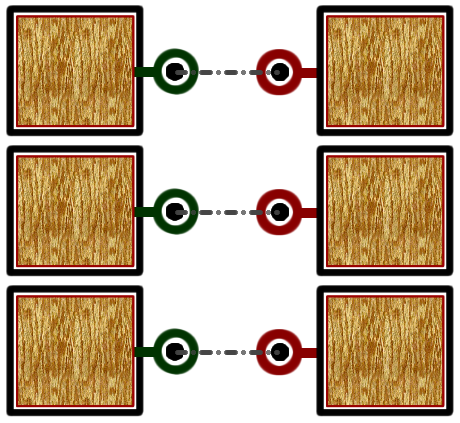
\includegraphics[width=0.25\textwidth]{comm_11.png}
}
\hspace{0.05\textwidth}%
\subfloat[][Communication 1 to N]{%
	\label{subfig:comm_diff}
	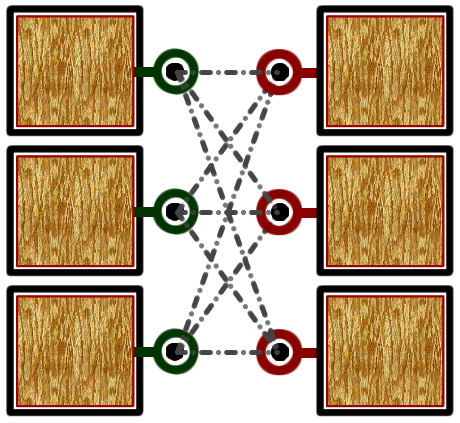
\includegraphics[width=0.25\textwidth]{comm_1n.png}
}
\hspace{0.05\textwidth}%
\subfloat[][Cyclic communication]{%
	\label{subfig:comm_ring}
	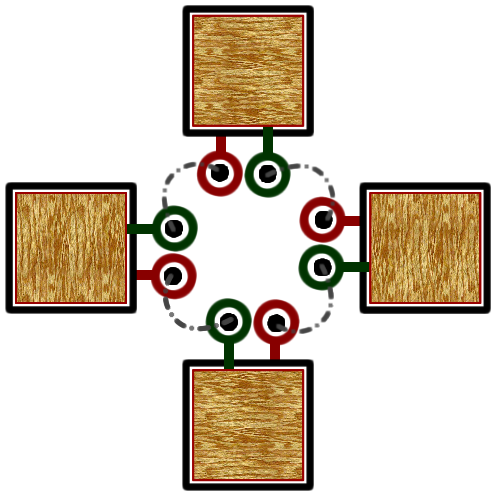
\includegraphics[width=0.25\textwidth]{comm_ring2.png}
}
\caption[]{Graphic representation of communication operators}
\label{fig:comm}
\end{figure}

\poslexample{These operators can be combined beteewn themself to contruct any kind of \comstr. Figure~\ref{fig:ex:comb} shows a simple example combining solvers doubly connected and non connected solvers. Assuming that all solvers $S_i, i\in[1..5]$ have a module $\mathcal{M}$ sent by a send operator, and a \opch{} $\mathcal{CM}$, the corresponding code is the following:
\begin{gather*}
\left[\mathcal{S}_1\cdot\mathcal{M}, \mathcal{S}_2\cdot\mathcal{M}, \mathcal{S}_{3}\cdot\mathcal{M}\right] \onetonsep \left[\mathcal{S}_4\cdot\mathcal{CM}, \mathcal{S}_5\cdot\mathcal{CM}\right]\\
\left[\mathcal{S}_4\cdot\mathcal{M}, \mathcal{S}_5\cdot\mathcal{M}\right] \onetoonesep \left[\mathcal{S}_1\cdot\mathcal{CM}, \mathcal{S}_{3}\cdot\mathcal{CM}\right]\\
\left[\mathcal{S}_6\right]\\
\left[\mathcal{S}_7\right]
\end{gather*}
}

\begin{figure}[h]
\centering
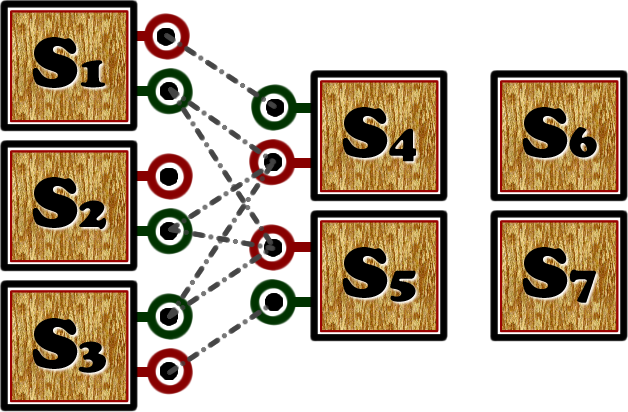
\includegraphics[width=0.35\textwidth]{ex_comb.png}
\caption[]{Graphic representation of communication operators}
\label{fig:ex:comb}
\end{figure}

\separation

%When we apply a connection operator $\circled{op}$ between a \jacks{} list $\mathcal{J}$ and a \outlets{} list $\mathcal{O}$, internally we are assigning an \textit{computation unit} (typically a thread) to each solver that we declare in each list. This assignment receives the name of \textit{Solver Scheduling}. Before running the \soset{}, this \textit{computation unit} is just an integer $\tau \in [0..N]$ identifying uniquely each of the solvers. When the \soset{} is launched, the solver with the identifier $\tau$ runs inside the computation unit $\tau$. This identifier assignation remains independent of the real availability of resources of computation. It just takes into account the user declaration. This means that, if the user declares 30 solvers (15 senders and 15 receivers) and the \soset{} is launched using 20 cores, only the first 20 solvers will be executed, and in consequence, there will be 10 solvers sending information to nowhere. Users should take this into account when declaring the \soset.

The connection process depends on the applied connection operator. In each case the goal is to assign, to the sending operator ($\senddataop{.}$ or $\sendmoduleop{.}$) inside the \as{}, the identifier of the solver (or solvers, depending on the connection operator) where the information will be sent. Algorithm~\ref{algo:connecting} presents the connection process.

\incmargin{1.4em}
\linesnumbered
\begin{algorithm}[H]
\dontprintsemicolon
\SetLine
\SetKwFor{While}{while}{do}{end}
\SetKwData{Jacks}{$\mathcal{J}$}
\SetKwData{Outlets}{$\mathcal{O}$}
\SetKwData{SS}{$S$}
\SetKwData{SSjack}{$S_{jack}$}
\SetKwData{RR}{$R$}
\SetKwData{RRoutlet}{$R_{outlet}$}
\SetKwData{RRid}{$R_{id}$}
\SetKwFunction{GetSolver}{GetSolverFromConnector}
\SetKwFunction{GetNext}{GetNext}
\SetKwFunction{Sched}{Schedule}
\SetKwFunction{Root}{root}
\SetKwFunction{Connect}{Connect}
\SetKwInOut{Input}{input}
\SetKwInOut{Output}{output}
\SetKw{KwTo}{int}

\Input{\Jacks list of \jacks{}, \\ \Outlets list of \outlets}
%\Output{\Q = $\left\{Q_i\right\}_{i=1\dots K}$: $K$ subsets of \Uni}
%\BlankLine
\While{no available jacks or outlets remain}{ %\nllabel{paso_condicion}
	\SSjack	$\leftarrow$ \GetNext{\Jacks}\;
	\RRoutlet $\leftarrow$ \GetNext{\Outlets}\;
	\SS $\leftarrow$ \GetSolver{\SSjack}\;	
	\RR $\leftarrow$ \GetSolver{\RRoutlet}\;
	%\Sched{\SS}\;
	%\RRid $\leftarrow$ \Sched{\RR}\;
	\Connect{\Root{\SS},\SSjack, \RR} %\RRid} %\label{step2} \tcc{It also removes the returned element}
}
\caption{Connection main algorithm}\label{algo:connecting}
\end{algorithm}

In Algorithm~\ref{algo:connecting}:
\begin{itemize}
\item \texttt{GetNext($\dots$)} returns the next available solver-jack (or solver-outlet) in the list, depending on the connection operator, e.g., for the connection operator One-to-N, each \jack{} in $\mathcal{J}$ must be connected with each \outlet{} in $\mathcal{O}$.
\item \texttt{GetSolverFromConnector($\dots$)} returns the solver name given a connector declaration.
%\item \texttt{Schedule($\dots$)} schedules a solver and returns its identifier.
\item \texttt{Root($\dots$)} returns the {\it root} \cm{} of a solver.
\item \texttt{Connect($\dots$)} %is presented in Algorithm~\ref{algo:connect}. It 
searches the \om{} $S_{jack}$ recursively inside the {\it root} \cm{} of $S$ and places the identifier $R_{id}$ into its list of destination solvers.
\end{itemize}

\poslexample{Let us suppose that we have declared two solvers $S$ and $Z$, both implementing the \as{} in Algorithm~\ref{algo:as_example}, so they can be either sender or receiver. The following code connects them using the operator {\bf 1~to~N}:
$$\left[S\cdot A\right] \onetonsep \left[Z\cdot C.M.\right]$$
If the operator {\bf 1~to~N} is used with only with one solver in each list, the operation is equivalent to applying the operator {\bf 1~to~1}. However, to obtain a communication strategy like the one showed in Figure~\ref{subfig:comm_diff}, six solvers (three senders and three receivers) have to be declared to be able to apply the following operation:
$$\left[S_1\cdot A, S_2\cdot A, S_3\cdot A\right]\onetonsep \left[Z_1\cdot C.M., Z_2\cdot C.M., Z_3\cdot C.M.\right]$$
\posl{} provides a mechanism to make this easier, through two {\it syntactic sugars} explained below.
}

%\subsection{Solver namespace expansion}
\separation

One of the goals of \posl{} is to provide a way to declare sets of solvers to be executed in parallel easily. For that reason, \posl{} provides two syntactic sugars %forms of namespace expansion, 
in order to create sets of solvers using already declared ones:
\begin{enumerate}
\item Using an integer to denote how many times a solver name will appear in the declaration.
\item Using an integer to denote how many times the connection will be repeated in the declaration.
\end{enumerate}

The following example explains clearly these syntactic sugars:

%\textbf{Solver name expansion - } Uses an integer $K$ to denote how many times the solver name $S$ will appear in the declaration. $\left[\dots S_i\cdot\mathcal{M}(K),\dots\right]$ expands as $\left[\dots S_i\cdot\mathcal{M}, S_i^2\cdot\mathcal{M},\dots S_i^K\cdot\mathcal{M}\dots\right]$\\
%and all new solvers $S_i^j, j\in [2..K]$ are created using the same solver declaration of solver $S_i$.

%\textbf{Connection declaration expansion - } Uses an integer $K$ to denote how many times the connection will be repeated in the declaration. Let 
%\begin{inparaenum}[a)]
%\item $\left[\mathcal{S}_1\cdot\mathcal{M}_1,\dots,\mathcal{S}_{N}\cdot\mathcal{M}_{N}\right]$ and 
%\item $\left[\mathcal{R}_1\cdot\mathcal{CM}_1,\dots,\mathcal{R}_{M}\cdot\mathcal{CM}_{M}\right]$ be the list of \jacks{} and \outlets, respectively, and
%\item $\circled{op}$ a connection operator.
%\end{inparaenum} Then $$\left[\mathcal{S}_1\cdot\mathcal{M}_1,\dots,\mathcal{S}_{N}\cdot\mathcal{M}_{N}\right] \poslop{op} \left[\mathcal{R}_1\cdot\mathcal{CM}_1,\dots,\mathcal{R}_{M}\cdot\mathcal{CM}_{M}\right]K$$ expands as
%
%\begin{align*}
%\left[\mathcal{S}_1\cdot\mathcal{M}_1,\dots,\mathcal{S}_{N}\cdot\mathcal{M}_{N}\right] &\poslop{op} \left[\mathcal{R}_1\cdot\mathcal{CM}_1,\dots,\mathcal{R}_{M}\cdot\mathcal{CM}_{M}\right]\\
%\left[\mathcal{S}_1^2\cdot\mathcal{M}_1,\dots,\mathcal{S}_{N}^2\cdot\mathcal{M}_{N}\right] &\poslop{op} \left[\mathcal{R}_1^2\cdot\mathcal{CM}_1,\dots,\mathcal{R}_{M}^2\cdot\mathcal{CM}_{M}\right]\\
%&\dots\\
%\left[\mathcal{S}_1^K\cdot\mathcal{M}_1,\dots,\mathcal{S}_{N}^K\cdot\mathcal{M}_{N}\right] &\poslop{op} \left[\mathcal{R}_1^K\cdot\mathcal{CM}_1,\dots,\mathcal{R}_{M}^K\cdot\mathcal{CM}_{M}\right]\\
%\end{align*}
%and all new solvers $S_i^k, i\in[1..N]$ and $R_j^k,j\in [1..M]$, $k\in[2..K]$, are created using the same solver declaration of solvers $S_i$ and $R_j$, respectively.

\poslexample{Suppose that I have created  solvers $S$ and $Z$ mentioned in the previews example. As a communication strategy, I want to connect them through the operator {\bf 1~to~N}, using $S$ as sender and $Z$ as receiver. Then,  %using \textbf{namespace expansions}, 
we need to declare how many solvers I want to connect. Algorithm~\ref{algo:comm_str_ex} shows the desired communication strategy. Notice in this example that the connection operation is affected also by the number $2$ at the end of the line. %, as {\bf connection declaration expansion}. 
In that sense, and supposing that 12 units of computation are available, a \soset{} working on parallel following the topology described in Figure~\ref{fig:ex_conn} can be obtained.}

\begin{algorithm}[H]
\dontprintsemicolon
\SetNoline
%\myproc{
[ S$\cdot A$ (3) ] $\onetonsep$ [ Z$\cdot C.M.$ (3) ] 2 ;
\caption{A communication strategy}\label{algo:comm_str_ex}
\end{algorithm}

\begin{figure}[h]
	\centering	
	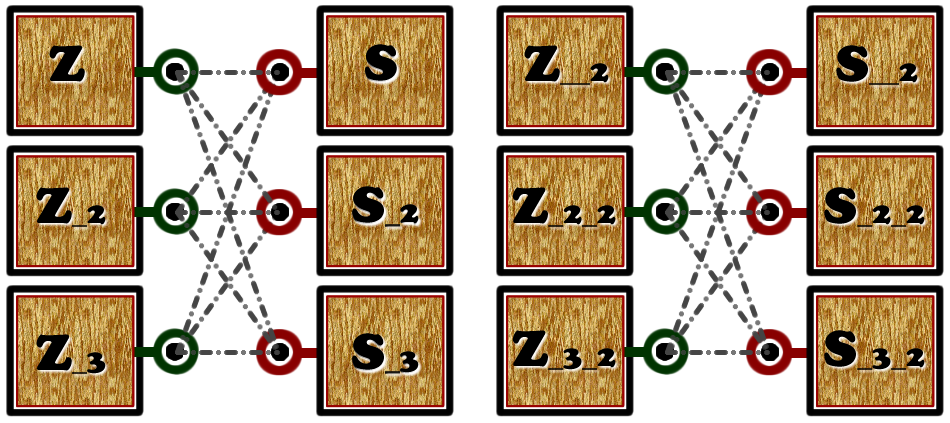
\includegraphics[width=0.6\linewidth]{ex_top.png}
	\caption{An example of connection strategy for 12 units of computation}\label{fig:ex_conn}
\end{figure}

\section{Summarize}
\label{sec:posl_zum}

In this chapter \posl{} have been formally presented, as a Parallel--Oriented Solver Language to build meta-heuristic-based solver to solve \CSPs{}. This language provides a set of \oms{} useful to solve a wide range of constrained problems. It is also possible to create new ones, through the low-level framework in C++ programming language. \posl{} also provides a set of \opchs{}, essential features to share information between solvers.

One of the \posl's advantages is the possibility of creating, using an operator-based language, \ass{} remaining independent from concrete \bothmodules{}. It is then possible to create many different solvers builded upon the same \as{} by only instantiating different modules. It is also possible to create different \comstrs{} upon the same \soset{} by using \commopers{} that \posl{} provides.

In the next chapter, a detailed study of various communicating and non-communicating strategies is presented using some \CSPs{} as benchmarks. %In this study, is showed the efficacy of \posl{} to analyze quickly and easily these strategies.